\documentclass[12pt]{beamer}
\usepackage[utf8]{inputenc}
\usepackage[T1]{fontenc}
\usepackage{lmodern}
\usepackage[spanish]{babel}
\usepackage{amsmath}
\usepackage{amsfonts}
\usepackage{amssymb}
\usepackage{graphicx}
\usepackage{hyperref}
%\usetheme{Boadilla}
\usetheme[block=fill]{metropolis}
\useoutertheme[]{}

\begin{document}
	\author{Fernando Oleo Blanco \\ fernando.oleo@alu.comillas.edu \hfill 	\href{https://github.com/Irvise/Documents}{github.com/Irvise/Documents}}
	\title{Introducción a Linux}
	%\subtitle{}
	%\logo{}
	\institute{ICAI - LinuxEC}
	\date{\today}
	%\subject{}
	%\setbeamercovered{transparent}
	\setbeamertemplate{navigation symbols}{}
	\setbeamertemplate{footline}[page number]
\begin{frame}[plain]
	\maketitle
\end{frame}

\begin{frame}{No se verá}
	\begin{itemize}
		\item \textbf{Herramientas *NIX estándar:} \texttt{*sh, vi(m), Emacs, awk, sed, make...}
		\item \textbf{Programación shell} \tiny lo siento por los de teleco \normalsize
		\item \textbf{Cualquier cosa relacionada a servidores:} \texttt{SSH, NGINX, Apache, CGI...}
		\item \textbf{Administración generalista:} \texttt{systemd, /etc, /proc, /var...}
		\item \textbf{Elementos ``micro'':} \texttt{Raspberry Pi, RTOS, /sys...}
	\end{itemize}
\end{frame}

\begin{frame}[allowframebreaks]{Índice}
	\tableofcontents
\end{frame}

\section{Historia}

\subsection{UNIX}
\begin{frame}{UNIX}
	\begin{block}{Inicios}
		Nacido a finales de los años 60, principios de los 70. Creado por Bell Labs, y uno de los grupos más dotados de la historia de la computación. Es la semilla de los OSs modernos.
	\end{block}
	\begin{columns}
		\begin{column}{0.5\textwidth}
			\begin{figure}
				\centering
				\href{http://cat-v.org/}{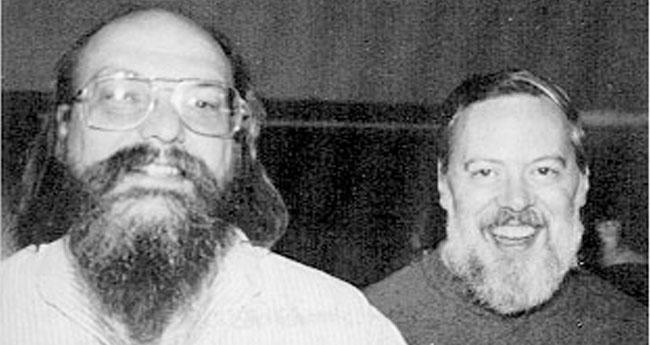
\includegraphics[width=\linewidth]{Ken-Thompson-og-Dennis-Ritchie}}
				\caption{Ken Thompson \& Dennis Ritchie (Creador de C)}
				\label{fig:ken-thompson-og-dennis-ritchie}
			\end{figure}
		\end{column}
		\begin{column}{0.5\textwidth}
			\begin{figure}
				\centering
				\href{https://www.youtube.com/watch?v=QFK6RG47bww&list=PLzH6n4zXuckqZ90zLyy36qjO5YIn1RulG}{\includegraphics[width=\linewidth]{Brian_Kernighan_in_2012_at_Bell_Labs_1}}
				\caption{Brian Kernighan}
				\label{fig:briankernighanin2012atbelllabs1}
			\end{figure}
		\end{column}
	\end{columns}
	
\end{frame}

\subsection{GNU/FSF}
\begin{frame}{GNU}
	\begin{block}{GNU}
		Stallman, trabajando en el MIT anuncia ``\textit{the GNU Proyect}" en 1983, en el 84 empieza su desarrollo. El objetivo es tener un sistema completamente \textbf{libre}; ver \href{https://www.gnu.org/gnu/manifesto.html}{\textit{GNU's Manifesto}}. \textit{GNU is Not UNIX}. 
	\end{block}
	\begin{columns}
		\begin{column}{0.5\textwidth}
			\begin{figure}
				\centering
				\href{https://www.stallman.org/}{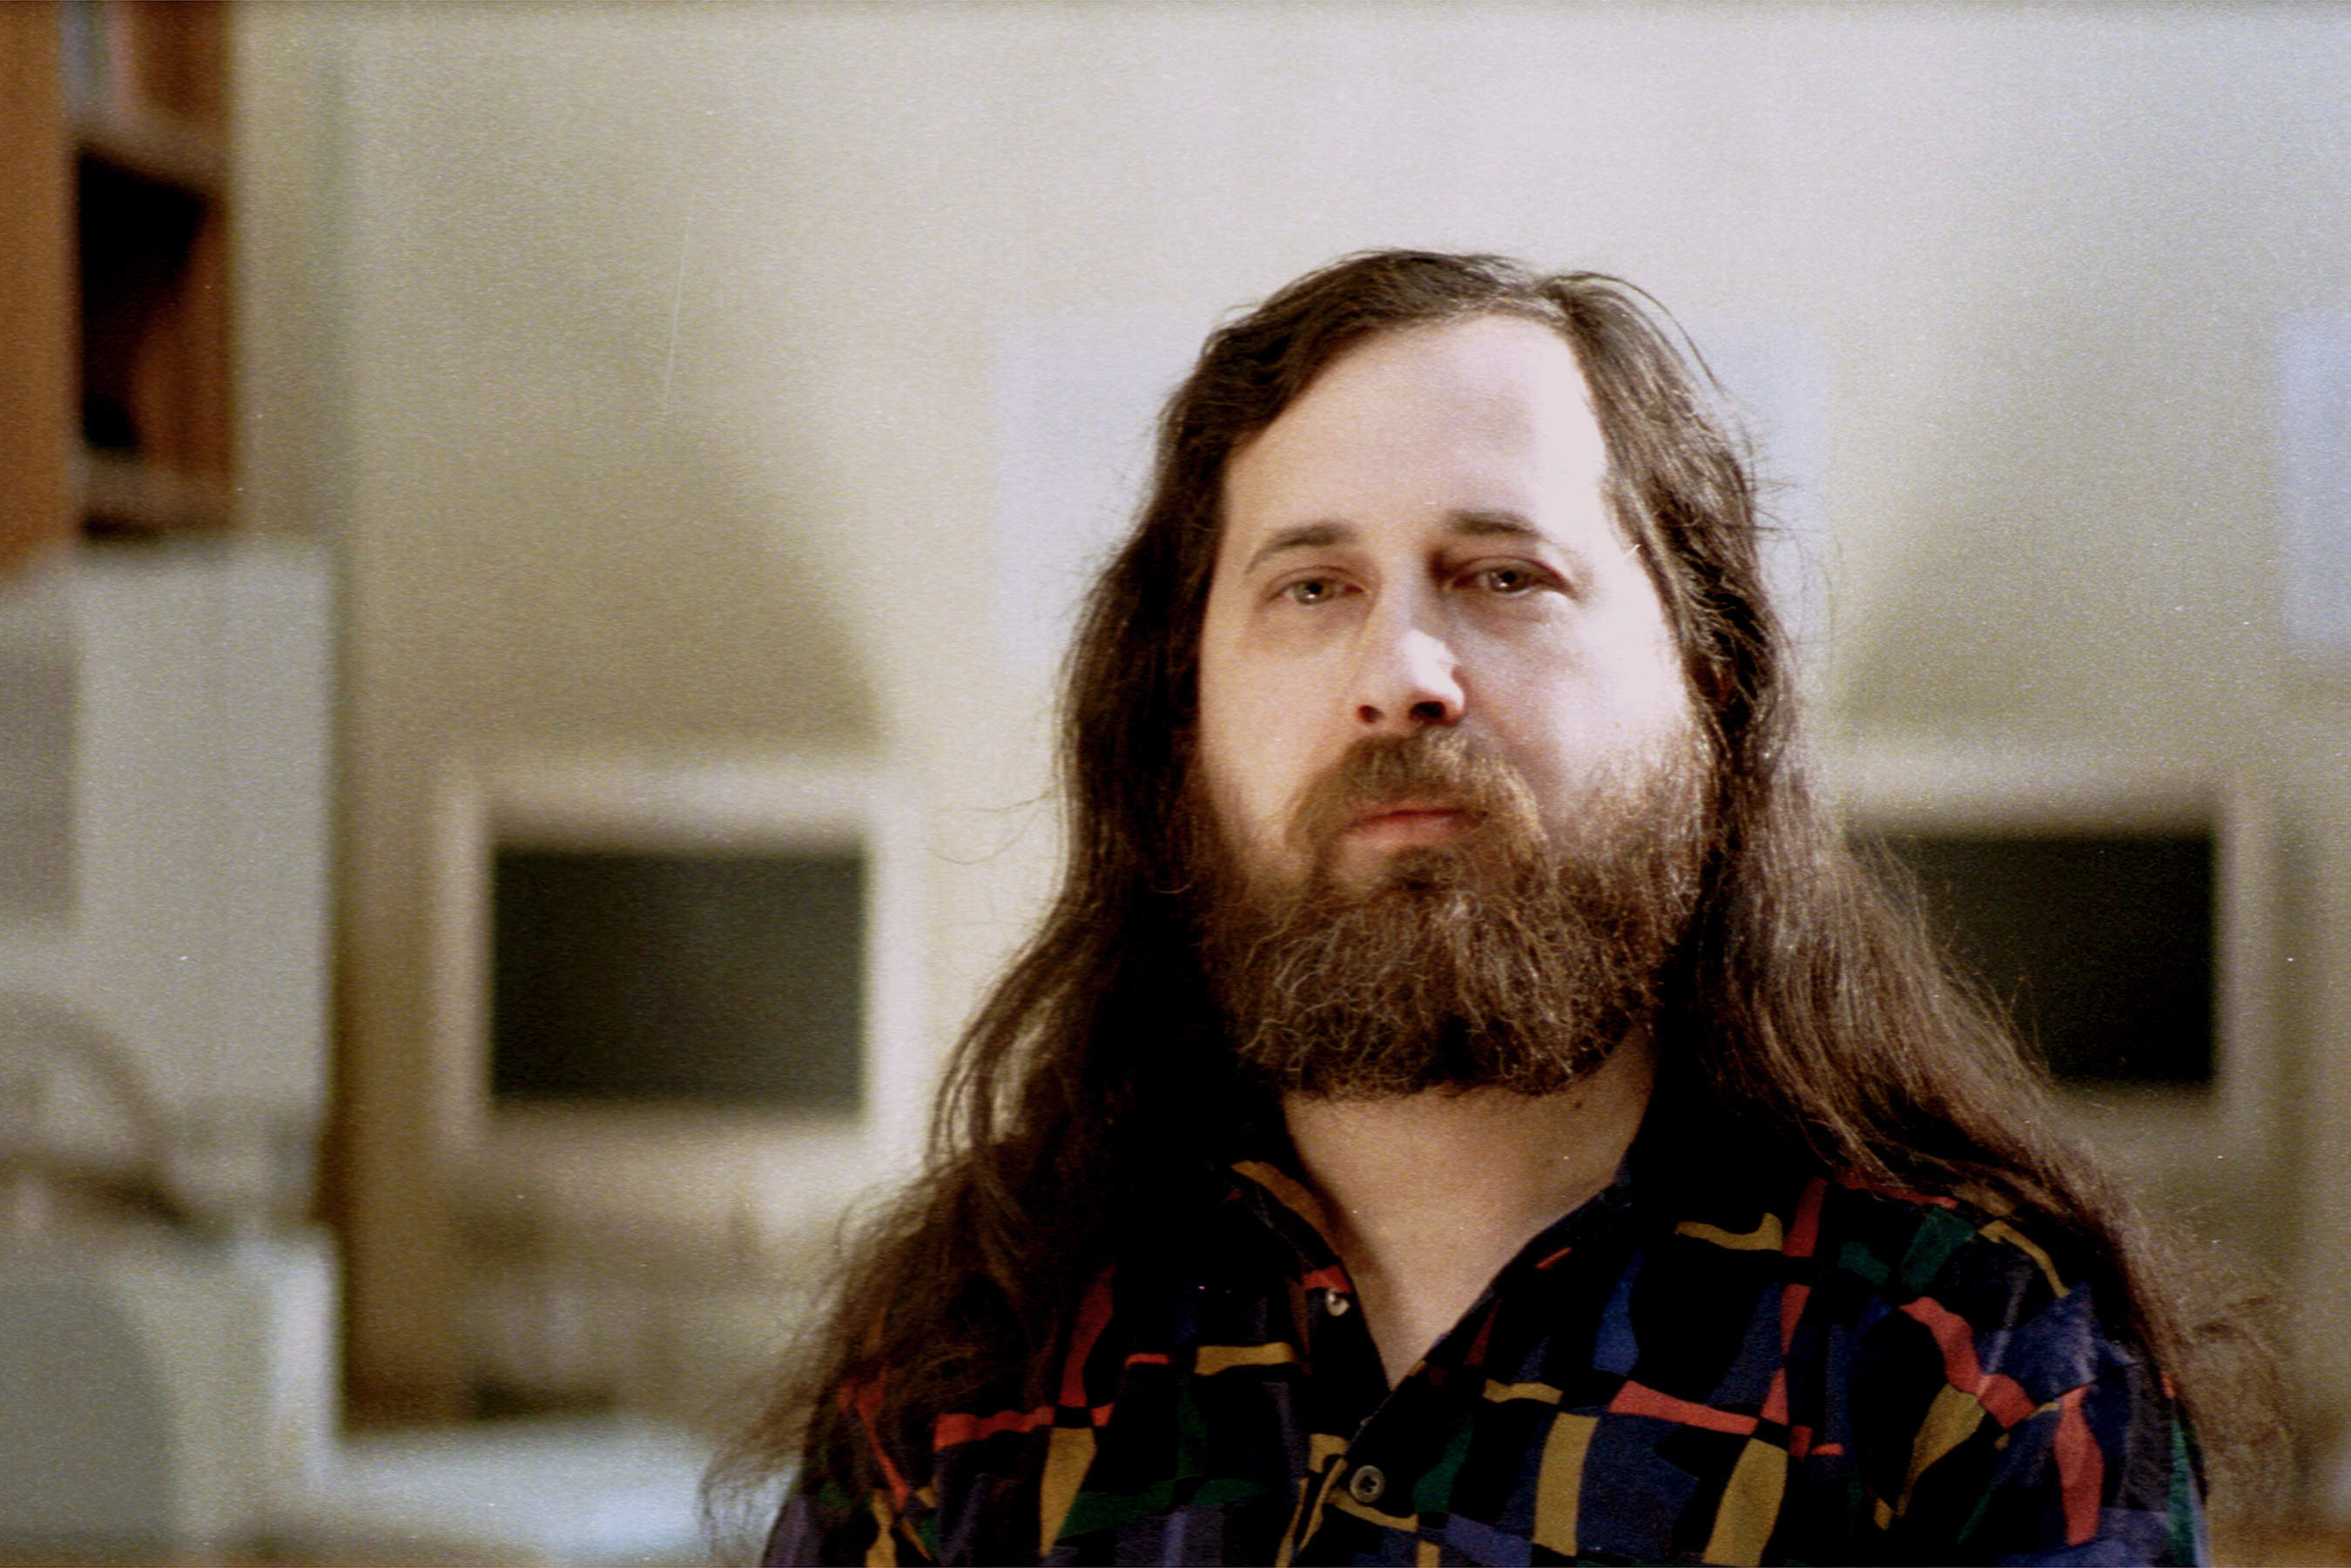
\includegraphics[width=\linewidth]{anopensourcelabel}}
				\caption{Richard Stallman}
				\label{fig:anopensourcelabel}
			\end{figure}
		\end{column}
		\begin{column}{0.5\textwidth}
			\begin{figure}
				\centering
				\href{https://www.youtube.com/watch?v=1jPmnDZ6ab8}{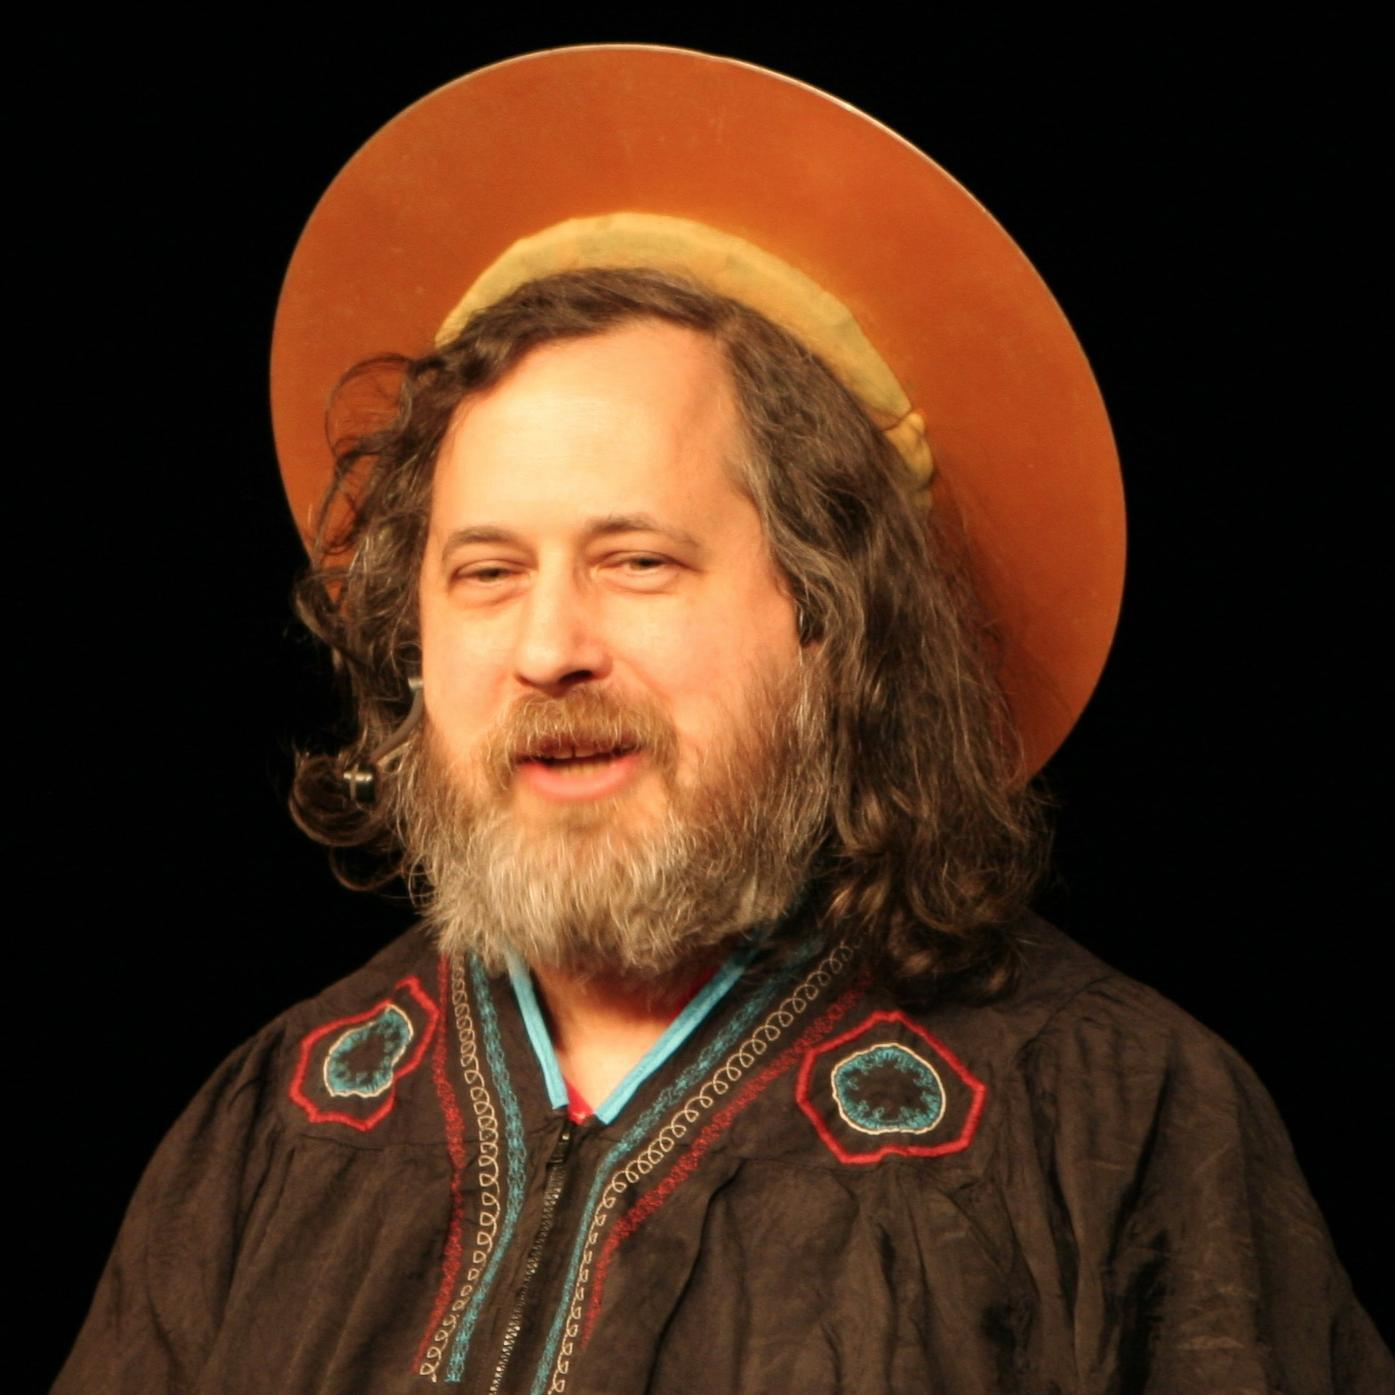
\includegraphics[width=0.7\linewidth]{FlICmGnj}}
				\caption{St. IGNcius}
				\label{fig:flicmgnj}
			\end{figure}
		
		\end{column}
	\end{columns}
\end{frame}

\begin{frame}{FSF}
	\begin{block}{Free Software Foundation}
		Fundación creada para la defensa del software \textbf{libre}. Da fondos a proyectos GNU, apoyo legal y hace campañas en contra de sus intereses y sirve como organismo \textit{regulador.}
	\end{block}
\begin{columns}
	\begin{column}{0.5\textwidth}
	\begin{figure}
		\centering
		\href{https://www.gnu.org/licenses/licenses.html}{
\includegraphics[width=0.5\linewidth]{gerwinski-gnu-head}}
		\caption{Logo GNU}
		\label{fig:gerwinski-gnu-head}
	\end{figure}
\end{column}
\begin{column}{0.5\textwidth}
	\begin{figure}
		\centering
		\href{https://www.fsf.org/}{
\includegraphics[width=0.7\linewidth]{fsf}}
		\caption{FSF}
		\label{fig:fsf}
	\end{figure}
	
\end{column}
\end{columns}

\end{frame}

\begin{frame}{Las cuatro libertades}
	\begin{itemize}
		\item[0] Libertad para usar el programa para lo que desees como lo desees.
		\item[1] Libertad para el estudio y la modificación del programa y que sean aplicables.
		\item[2] Libertad para distribuir copias para ayudar a terceros.
		\item[3] Libertad par distribuir copias modificadas a terceros.
	\end{itemize}
\vfill
\centering{\Large ¡Software libre no significa \textit{no comercial}!}
\vfill
\href{https://www.gnu.org/licenses/license-list.html}{Link: Lista de licencias}
\end{frame}

\subsection{Linux}
\begin{frame}{Linux}
	1987, MINIX es lanzado con la intención de ser un OS para la enseñanza. De código abierto, pero no distribuible ni modificable. No hay sistemas operativos (buenos) disponible para i386.
	\begin{block}{Hace muchos años, en un lugar muy remoto... (Helsinki)}
	Al no poder modificar MINIX para su nuevo ordenador AT, Linus Torvalds decide crear su propio OS en imagen a MINIX usando, por completo, software GNU. El 25 de Agosto 1991, se publica \textit{the "Linux" manifesto.} En 1992 se licencia oficialmente bajo la GPLv2.
	\end{block}
\end{frame}

\begin{frame}
	\begin{columns}
		\begin{column}{0.5\linewidth}
			\begin{figure}
				\centering
				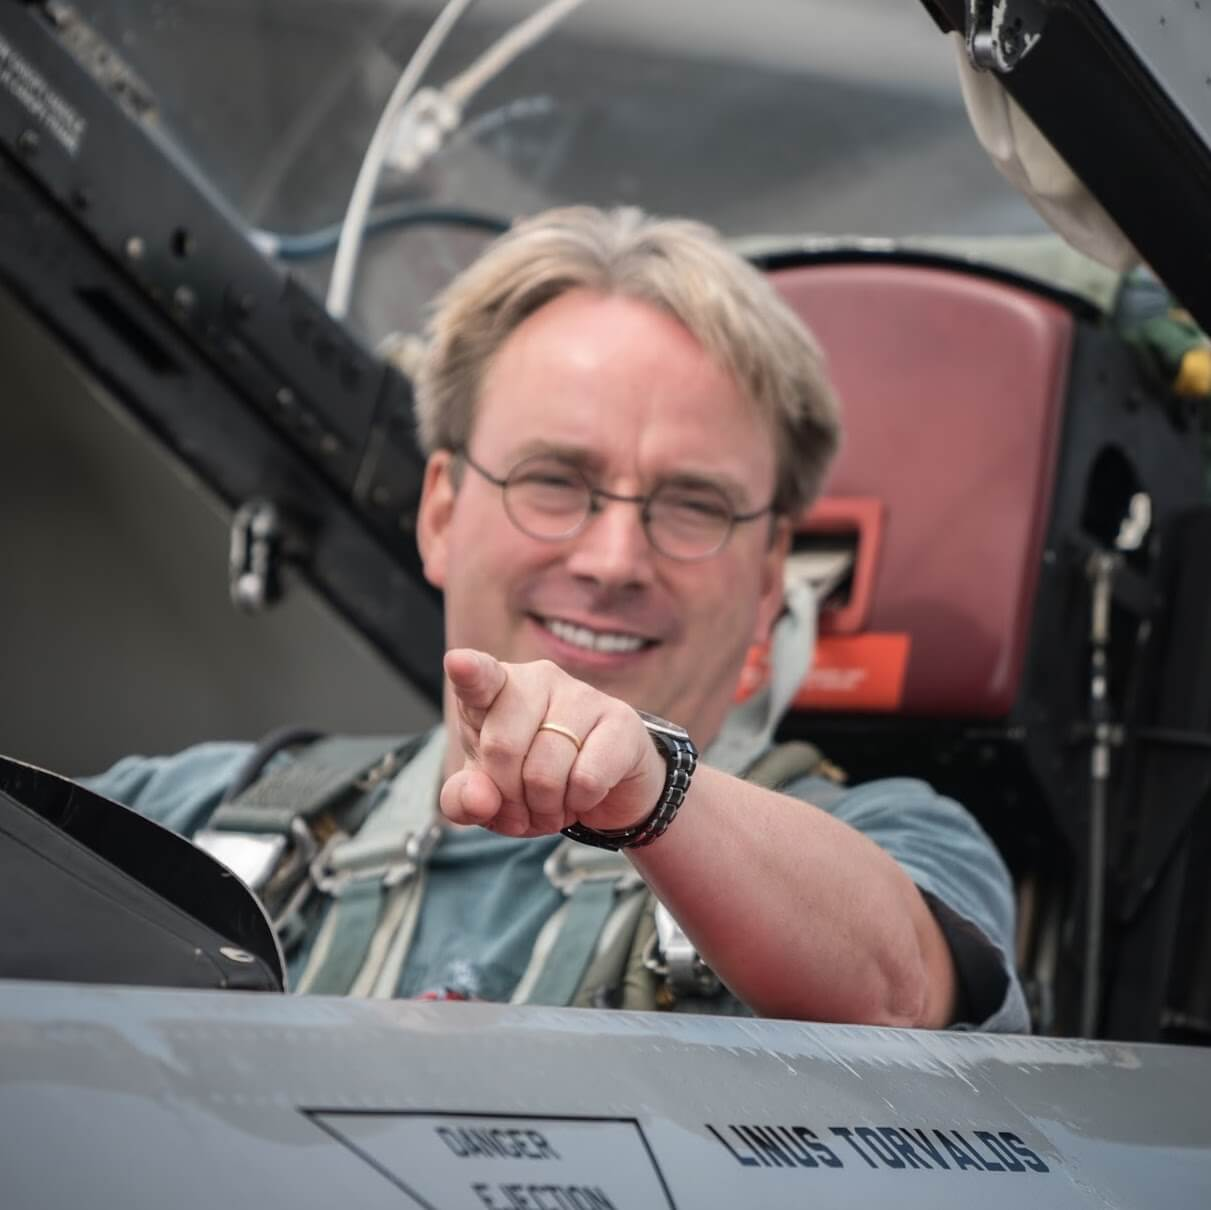
\includegraphics[width=\linewidth]{Linus-Torvalds}
				\caption{Linus Torvalds}
			\end{figure}
		\end{column}
		\begin{column}{0.5\linewidth}
			\begin{figure}
				\centering
				
\includegraphics[width=0.9\linewidth]{linux_PNG5}
				\caption{Tux, la mascota}
			\end{figure}
		\end{column}
	\end{columns}
\end{frame}

\section{Distribuciones/\textit{Distros}}
\begin{frame}{Distibuciones/\textit{Distros}}
	\begin{block}{¿Pero qué es Linux?}
		Es un \textit{KERNEL.} Es el pegamento entre el \textit{hardware} (parte física) y el \textit{software} (código) en un ordenador. Administra los recursos, por ejemplo, la memoria que un programa puede usar; implementa sistemas seguros, protocolos, control directo del hardware, etc.
	\end{block}
	\begin{block}{Distros}
		Son ``empaquetamientos'' del kernel Linux con herramientas administrativas, programas, etc; de carácter específico.
	\end{block}
\end{frame}

\begin{frame}{Distros, \textit{clasificación}}
	Las \textit{distros} se crean siguiendo criterios de necesidad y objetivos:
	\begin{itemize}
		\item \textbf{Estabilidad:} servidores, ordenadores millonarios o PCs normales. La diferencia principal es cómo de moderno es el software.
		\item \textbf{Objetivo:} ser fácil de usar, flexible, que corra en dispositivos de potencia limitada, etc.
		\item \textbf{Administración:} automatizada, simple, manual, profunda, declarativa, etc.
		\item \textbf{\textit{Facilidad de uso:}} suits completas de software, compatibilidades, entornos gráficos, etc.
	\end{itemize}
\end{frame}

\begin{frame}{Familias más conocidas}
\vspace*{-2em}
\begin{figure}
	\begin{tabular}{cccc}
		Familias & RedHat \newline CentOS & OpenSUSE & Debian \\ \hline
		& CentOS & Leap & Debian \\
		\textit{Estables} &
\includegraphics[scale=0.3]{centos_logo_blue} & 
\includegraphics[scale=0.16]{leap-500-500x500} & 
\includegraphics[scale=0.07]{Debian-Logo-Vector}\\
		Diarias & \includegraphics[scale=0.01]{fedora-logo} & 
\includegraphics[scale=0.6]{opensuse-tumbleweed-logo} & 
\includegraphics[scale=0.07]{logo-ubuntu} \\ 
		& Fedora & Tumbleweed & Ubuntu
	\end{tabular}
\end{figure}
\end{frame}

\begin{frame}{Si por elegir...}
	\begin{figure}
		\centering
		
\includegraphics[width=0.77\linewidth]{distros-1024x768}
		\caption{Comunidad *NIX}
\end{figure}
	
\end{frame}

\section{Instalación}
\begin{frame}{Instalación}
	\textit{Checklist}
	\begin{itemize}
		\item Desfragmentar Windows. Hacer partición desde Windows. Desactivar fastboot.
		\item Tendremos que seleccionar en la BIOS/UEFI (F2, F10, F12) en el arranque, que use el CD/USB
		\item Comprobar si el PC usa BIOS o (U)EFI. Ubuntu nos lo dirá.
		\begin{itemize}
			\item Si (U)EFI, tendremos que hacer una partición extra, formateada a FAT32 y \textit{label: boot}. Montada como \textit{/boot/efi}. Si Windows ya la creó, la seleccionamos. \textbf{¡Pero no la formateamos!}
		\end{itemize}
		\item Si el SSD/HDD usa la tabla de partición GPT, tenemos que dejar 2Mb libres en los primeros anillos. $\leftarrow$ \textbf{MUY ``raro''.}
		\item Proceder con la instalación con calma y revisando todo. No vendría mal comprobar el disco con \texttt{gparted}.
	\end{itemize}
\end{frame}

\begin{frame}{Posibles problemas}
	$\bullet$ \textbf{Gráficos:} los portátiles con tarjetas NVIDIA dan muchos problemas. Se recomienda instalar los drivers del fabricante (NVIDIA), si dan problemas, usar los drivers libres.\\
	\hfill \texttt{sudo ubuntu-drivers autoinstall}
	
	$\bullet$ \textbf{Batería:} ha mejorado muy notablemente en las últimas versiones, pero se recomienda instalar TLP.\\
	\hfill \texttt{sudo apt install tlp}
	
	$\bullet$ \textbf{Arranque de la instalación, problemas varios:} desactivar \texttt{ACPI, modeset} y arrancar en modo seguro.
\end{frame}

\begin{frame}{Práctica}
	\centering{\Huge A INSTALAR\normalsize}
\end{frame}

\begin{frame}{Instalación en equipos reales}
	\centering{\LARGE{Leer muy bien la documentación de la instalación de cada distribución. \\ \vspace{3em} Avisadme. No corrijo errores, ni aseguro nada.}}
\end{frame}

\section{Uso}
\begin{frame}[allowframebreaks]{Herramientas a tener en cuenta}
	\begin{block}{Package Manager. En Ubuntu: \texttt{apt}}
		Administra \textbf{TODO} nuestro software, obtiene el software desde \textit{repositorios} tanto predeterminados como añadidos. Nos centraremos en la instalación, eliminación y búsqueda de software en Ubuntu:
		\begin{itemize}
			\item \textbf{Actualizar} \texttt{sudo apt update \&\& sudo apt upgrade}
			\item \textbf{Instalar} \texttt{sudo apt install} \textit{software}
			\item \textbf{Eliminar} \texttt{sudo apt remove} \textit{software}
			\item \textbf{Buscar} \texttt{apt search} \textit{software}
		\end{itemize}
	\end{block}
	Otros \textit{package managers:}
	\begin{itemize}
		\item \textbf{Fedora:} \texttt{dnf}
		\item \textbf{OpenSUSE:} \texttt{zypper/Yast}
		\item \textbf{CentOS:} \texttt{yum}
		\item \textbf{Debian:} \texttt{apt-get*}
	\end{itemize}
	\begin{block}{Ayudas para un trabajo sencillo}
		En Ubuntu existe también la posibilidad de usar software gráfico:
		\begin{itemize}
			\item \textbf{Software Centre:} ya instalado, muy fácil y claro, \textbf{recomendado}.
			\item \textbf{Synaptic:} control más fino de todo el software.
		\end{itemize}
	\end{block}
\end{frame}

\subsection{Continuará}
\begin{frame}[allowframebreaks]{Para seguir aprendiendo: ayuda e información}
	\begin{block}{¡¡¡Wikis!!!}
		\begin{itemize}
			\item \textbf{Ubuntu:} \href{https://wiki.ubuntu.com/}{https://wiki.ubuntu.com/}
			\item \textbf{Arch Linux:} \href{https://wiki.archlinux.org/}{https://wiki.archlinux.org/}, es la más completa, pero requiere experiencia.
			\item El de la distribución que estéis usando.
			\item \textbf{Cualquier motor de búsqueda}
		\end{itemize}
	\end{block}
	\begin{block}{Foros}
		\begin{itemize}
			\item \textbf{Ubuntu:} \href{https://ubuntuforums.org/}{https://ubuntuforums.org/}
			\item \textbf{Archlinux:} \href{https://bbs.archlinux.org/}{https://bbs.archlinux.org/}, técnico igualmente.
			\item El de la distribución que estéis usando.
			\item \textbf{Cualquier motor de búsqueda}
		\end{itemize}
	\end{block}
\end{frame}

\begin{frame}{Temas que aprender}
	\begin{itemize}
		\item \textbf{Text editors:} \texttt{vi(m), Emacs}
		\item \textbf{Herramientas estándar:} \texttt{Shell, sed, patch, diff, make...}
		\item \textbf{Herramientas (tremendamente) útiles:} \texttt{git, rsync, VBOX/virt-manager...}
		\item \textbf{FS:} \texttt{/proc, /sys...}
		\item \textbf{Servidores:} \texttt{SSH, NGINX, logging...}
	\end{itemize}
\end{frame}

\begin{frame}{Fin}
	\centering{\Huge ¿Preguntas?\normalsize \vfill LINUXEC te necesita \\ fernando.oleo@alu.comillas.edu \\ \vfill \small Recuerdo que daré una charla de \LaTeXe, atentos a las pantallas}
	
\end{frame}

\end{document}